\documentclass[a4paper,12pt]{article}

\usepackage[T2A]{fontenc}
\usepackage[utf8]{inputenc}
\usepackage[english,russian]{babel}
\usepackage{amsmath}
\usepackage{pgfplots}
\usepackage{geometry}
\usepackage{graphicx}
\usepackage[section,above,below]{placeins}
\usepackage{afterpage,placeins}
\usepackage{booktabs}
\usepackage{listings}
\usepackage{color}

\usepackage{algorithm}
\usepackage[noend]{algpseudocode}

\DeclareGraphicsExtensions{.png,.jpg}

\geometry{left=2cm}
\geometry{right=1.5cm}
\geometry{top=1cm}
\geometry{bottom=1.5cm}

\headheight = 1cm
\footskip = 0.5cm

\parskip = 4.25mm % расстояние между строками
\parindent=6.375mm % расстояние между абзацами
\floatname{algorithm}{Алгоритм} % переопределение имени в псевдокоде

\begin{document}
    \begin{titlepage}
        \begin{center}
            \large
            Государственное образовательное учреждение высшего  образования\\
            “Московский государственный технический университет имени Н.Э.Баумана”
            \vspace{3cm}
            
            \textsc{Дисциплина: Анализ алгоритмов}
            \vspace{0.5cm}
                
            \textsc{Лабораторная работа №6}
            \vspace{3cm}
            
            {\LARGE Муравьиный алгоритм}
            \vspace{3cm}
            
            Студент группы ИУ7-54Б,\\   
            Котов Никита
            \vfill
            
            2019 г.            
            \end{center}
    \end{titlepage}
    
    \begin{center}
    	\tableofcontents
    \end{center}
	
	\setcounter{page}{2}
	\newpage
    \begin{center}
        \section*{Введение}
        \addcontentsline{toc}{section}{Введение}
    \end{center}
        \label{sec:intro}
\quad 
Муравьиный алгоритм - алгоритм для нахождения приближённых решений задач оптимизации на графах, таких, как задача коммивояжера, транспортная задача и аналогичных задач поиска маршрутов на графах. 
Муравья нельзя назвать сообразительным. Отдельный муравей не в состоянии принять ни малейшего решения. Дело в том, что он устроен крайне примитивно: все его действия сводятся к элементарным реакциям на окружающую обстановку и своих собратьев. Муравей не способен анализировать, делать выводы и искать решения.

Эти факты, однако, никак не согласуются с успешностью муравьев как вида. Они существуют на планете более 100 миллионов лет, строят огромные жилища, обеспечивают их всем необходимым и даже ведут настоящие войны. В сравнении с полной беспомощностью отдельных особей, достижения муравьев кажутся немыслимыми.

Добиться таких успехов муравьи способны благодаря своей социальности. Они живут только в коллективах – колониях. Все муравьи колонии формируют так называемый роевой интеллект. Особи, составляющие колонию, не должны быть умными: они должны лишь взаимодействовать по определенным – крайне простым – правилам, и тогда колония целиком будет эффективна.

В колонии нет доминирующих особей, нет начальников и подчиненных, нет лидеров, которые раздают указания и координируют действия. Колония является полностью самоорганизующейся. Каждый из муравьев обладает информацией только о локальной обстановке, не один из них не имеет представления обо всей ситуации в целом – только о том, что узнал сам или от своих сородичей, явно или неявно. На неявных взаимодействиях муравьев, называемых стигмергией, основаны механизмы поиска кратчайшего пути от муравейника до источника пищи.

Каждый раз проходя от муравейника до пищи и обратно, муравьи оставляют за собой дорожку феромонов. Другие муравьи, почувствовав такие следы на земле, будут инстинктивно устремляться к нему. Поскольку эти муравьи тоже оставляют за собой дорожки феромонов, то чем больше муравьев проходит по определенному пути, тем более привлекательным он становится для их сородичей. При этом, чем короче путь до источника пищи, тем меньше времени требуется муравьям на него – а следовательно, тем быстрее оставленные на нем следы становятся заметными.

В 1992 году в своей диссертации Марко Дориго (Marco Dorigo) предложил заимствовать описанный природный механизм для решения задач оптимизации [1]. Имитируя поведение колонии муравьев в природе, муравьиные алгоритмы используют многоагентные системы, агенты которых функционируют по крайне простым правилам. Они крайне эффективны при решении сложных комбинаторных задач – таких, например, как задача коммивояжера, первая из решенных с использованием данного типа алгоритмов.
\\ \\*
		Цель лабораторной работы: изучить муравьиный алгоритм на материале решения задачи Коммивояжера \\*
В рамках выполнения работы необходимо решить следующие задачи:
		\begin{itemize}
			\item дать постановку задачи;
			\item описать методы полного перебора и эвристический, основанный на муравьином алгоритме;
			\item реализовать данные методы;
			\item выбрать и подготовить классы данных;
			\item провести параметризацию метода, основанного на муравьином алгоритме;
			\item интерпретировать результаты и сравнить их с результатами метода полного перебора.
		\end{itemize}
    \newpage

    \begin{center}
        \section{Аналитическая часть}
	    \subsection{Описание алгоритмов}
    \end{center}
\subsubsection{Алгоритм полного перебора}


Алгоритм полного перебора для решения задачи коммивояжера предполагает рассмотрение всех возможных путей в графе и выбор наименьшего из них.

Такой подход гарантирует точное решение задачи, однако, так как задача относится к числу трансвычислительных, то уже при небольшом числе городов решение за приемлимое время невозможно.

\subsubsection{Муравьиный алгоритм}

Идея алгоритма основана на принципе работы колонии муравьев \cite{litlink3}. Колония муравьев рассматривается как многоагентная система, в которой каждый агент (муравей) функционирует автономно по очень простым правилам. В противовес почти примитивному поведению агентов, поведение всей системы получается разумным.
			 
			 Каждый муравей определеяет для себя маршрут, который необходимо пройти на основе феромона, который он ощущает, во время прохождения, каждый муравей оставляет феромон на своем пути, чтобы остальные муравьи могли по нему ориентироваться. В результате при прохождении каждым муравьем различного маршрута наибольшее число феромона остается на оптимальном пути. 			 \\			 
			 Самоорганизация колонии является результатом взаимодействия следующих компонентов:			 
			 \begin{itemize}
			 	\item случайнонсть -- муравьи имеют случайную природу движения;
			 	\item многократность -- колония допускает число муравьев, достигающее от нескольких десятков до миллионов особей;
			 	\item положительная обратная связь -- во время движения муравей откладывает феромон, позволяющий другим особям определить для себя оптимальный маршрут;
			 	\item отрицательная обратная связь - по истечении определенного времени феромон испаряется;
			 	\item целевая функция. 
			 \end{itemize}

Пусть муравей обладает следующими характеристиками: 
		 	\begin{itemize}
		 		\item зрение - определяет длину ребра;
		 		\item обоняние - чувствует феромон;
		 		\item память - запоминает маршрут, который прошел.
		 	\end{itemize}
	 	\noindent
	 	1) Введем целевую функцию $  \eta_{ij} = 1 / D_{ij} $, где $ D_{ij} $ - расстояние из текущего пункта i до заданного пункта j. \\*
	 	2) Считаются вероятности перехода в заданную точку по формуле (\ref{possibility}): 
	 	\begin{equation}\label{possibility}
	 		P_{kij} = 
	 		\begin{cases}
		 		\frac{t_{ij}^{a}\eta_{ij}^{b}}{\sum_{q=1}^m t^{a}_{iq}\eta^{b}_{iq}}, \textrm{\textit{вершина не была посещена ранее муравьем k,}} \\
		 		0, \textrm{\textit{иначе}}
		 	\end{cases}
	 	\end{equation}
		 	  
		где $ a, b $ -- настраиваемые параметры, $ t $ - концентрация феромона, причем $ a + b = const $, а при $ a = 0 $ алгоритм вырождается в жадный.
		
		3) Когда все муравьи завершили движение происходит обновление феромона по \\формуле (\ref{pheromone1}):
		
		\begin{equation}\label{pheromone1}
			t_{ij}(t+1) = (1-p)t_{ij}(t) + \varDelta t_{ij}, \varDelta t_{ij} = \sum_{k=1}^N t_{kij}
		\end{equation}
		\noindent где 
		\begin{equation}\label{pheromone2}
			\varDelta t_{kij} = 
			\begin{cases}
				Q/L_{k},   \textrm{\textit{ребро посещено k-ым муравьем,}}\\
				0, \textrm{\textit{иначе}}
			\end{cases}
		\end{equation}
		$ L_{k} $ -- длина пути k-ого муравья, $ Q $ -- настраивает концентрацию нанесения/испарения феромона, $N$ -- количество муравьев. 

	\begin{center}
	\subsection{Вывод по аналитическому разделу}
	\end{center}	
	По итогам аналитического раздела были описаны алгоритмы полного перебора и муравьиный алгоритм.

    \newpage

    \begin{center}
        \section{Конструкторская часть}
        \subsection{Разработка алгоритмов}
    \end{center}
    \subsubsection{Алгоритм полного перебора}
    
    В листинге 1 приведен псевдокод алгоритма полного перебора для решения задачи коммивояжера.
\floatname{algorithm}{Листинг}
\begin{algorithm}
		\caption{Алгоритм полного преебора для решения задачи коммивояжера $ex\_search(G, E)$}
		\begin{algorithmic}
			\State $best\_path\_len \gets -1$
			\State $queue \gets (0, 0)$
			\While{$ \text{queue is not empty} $}
				\State $ u <- queue.pop() $
				\For{$v \text{ } in \text{ } E(u[u.size()-1])$}
					\If {$v \text{ } in \text{ } u$}
						\State $continue$
					\EndIf
					\State $ new\_path \gets u $
					\State $ new\_path.add(v) $
					\State $ update\_best\_path $
				\EndFor
			\EndWhile								
		\end{algorithmic}
	\end{algorithm}	
	
	\newpage
    \subsubsection{Муравьиный алгоритм}
    
    Алгоритм разбит на следующие этапы: 
		\begin{itemize}
			\item день - на этом этапе муравьи совершают обход по карте и прокладывают путь;
			\item ночь - этап обновления феромона, наступает после завершения работы последнего муравья.
		\end{itemize}	

			 На рис. \ref{pic:ant_schema} отображена работа одного муравья.
			 \begin{figure}[H]	
			 	{
			 		\centering
			 		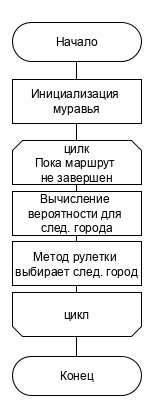
\includegraphics[scale=0.75]{ant.jpg}
			 		\caption{Схема работы одного муравья.}
			 		\label{pic:ant_schema}
			 	}
			 \end{figure}
		 
		 \noindentОписание этапов: 
		 \begin{itemize}
		 	\item инициализация муравья - установка муравья в стартовый город;
		 	\item цикл продолжает работу до тех пор, пока все вершины не будут посещены, внутри тела цикла высчитывается вероятность посещения следующего города по формуле (\ref{possibility}). Для определения конкретного города применяется метод рулетки, в котором случайно выбирается значение $ 0, \dots , 1 $ и на основе полученного значения с учетом вероятностей перехода в енпосещенные города определяется следующий город.
		 \end{itemize}
	\newpage
			Описанный выше алгоритм применяется N раз, где N -- количество вершин. Каждый муравей помещается в отдельную вершину на карте, после чего ищет маршрут. Когда последний муравей завершил обход всех вершин, производится поиск оптимального из полученных маршрутов, после чего феромон обновляется и в случае, если полученный результат не удовлетворяет поставленной задаче, алгоритм запускается заново. 
		

			\noindentНиже представлена работа на рис.\ref{pic:antalg_schema} алгоритма для всей колонии. 
			
			\begin{figure}[H]	
				{
					\centering
					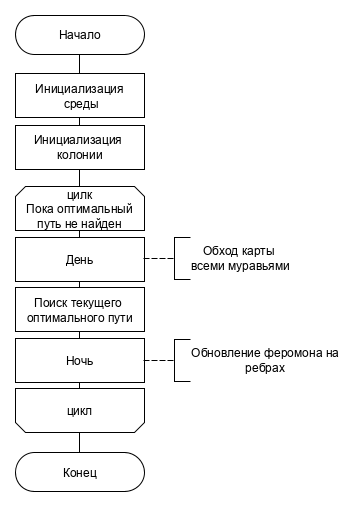
\includegraphics[scale=0.75]{ant_alg.png}
					\caption{Схема работы колонии.}
					\label{pic:antalg_schema}
				}
			\end{figure}
    
    \begin{center}
    	\subsection{Выводы по конструкторскому разделу}    
    \end{center}
   
    	\quad В результате работы над конструкторским разделом была разработана схемы алгоритма полного перебора и муравьиного алгоритма.
    	
    \newpage
    
    \begin{center}
     	\section{Технологическая часть}
        \subsection{Средства реализации}    
    \end{center}
    
		В качестве языка программирования был выбран C++, так как он предоставляет широкие возможности для эффективной реализации алгоритмов. 
	
	\begin{center}
	\end{center}
	\begin{center}
	        	\subsection{Требования к программному обеспечению}		
	\end{center}

			Программа должна обрабатывать матрицу смежностей методами полного перебора и эвристическим, основанным на муравьином алгоритме, подбирать параметры, на основе которых производятся оптимальные вычисления, выводить заданную матрицу смежностей, результат работы полного перебора и муравьиного алгоритма. 
	\begin{center}
	\end{center}
	\newpage			
    \begin{center}
        \subsection{Листинг кода}    
    \end{center}
				\lstset{
	        		language=C++,
	        		basicstyle=\ttfamily,
	        		keywordstyle=\color{blue}\ttfamily,
	        		stringstyle=\color{red}\ttfamily,
	        		commentstyle=\color{green}\ttfamily,
	        		morecomment=[l][\color{magenta}]{\#},
	        		columns=fullflexible,
	        	    tabsize=1, 
	        		breakatwhitespace=true
	        	}
        	
 В листингах 1 и 2 представлен код алгоритма полного перебора и класса колонии соответственно.
\begin{lstlisting}[frame=single,caption=Алгоритм полного перебора, breaklines]
std::pair<Path, float> exhaustive_search(const Graph &graph) {
    Path best_path(graph.size());
    float best_path_len = -1;
    std::vector<size_t> empty_v;
    std::queue<std::vector<size_t>> queue;
    queue.push(std::vector<size_t>(1, 0));

    while (!queue.empty()) {
        std::vector<size_t> u = queue.front();
        queue.pop();
        for (auto v: graph.getAvailableVertexes(u[u.size()-1] , empty_v)) {
            if (std::find(u.begin(), u.end(), v) == u.end()) {
                std::vector<size_t> new_path(u.size());
                std::copy(u.begin(), u.end(), new_path.begin());
                new_path.push_back(v);
                if (new_path.size() == graph.size()) {
                    auto len = path_len(graph, new_path);
                    if (len < best_path_len || best_path_len == -1) {
                        best_path_len = len;
                        best_path = new_path;
                    }
                } else {
                    queue.push(new_path);
                }
            }
        }
    }

    return std::make_pair(best_path, best_path_len);
}
\end{lstlisting}
\newpage
\begin{lstlisting}[frame=single,caption=Класс муравьиной колонии, breaklines]
struct Parameters {
    float a;
    float b;
    float p;
    float q;
    size_t times;
};

struct SimulationResult {
    std::vector<size_t> path;
    size_t days;
    float path_len;
};

class Colony {
public:
    explicit Colony(Graph &graph);
    SimulationResult simulation(Parameters parameters, size_t days);
private:
    static constexpr const float START_PHEROMONE = 0.3f;

    std::default_random_engine generator;
    std::uniform_real_distribution<float> distribution = std::uniform_real_distribution<float>(0, 1);

    Graph _graph;
    Graph _pheromone_graph;
    Parameters _parameters;

    std::pair<std::vector<size_t>, float> antAlgorithm(size_t start_vert);
    float random_probability();
    std::vector<float> vertexes_probabilities(size_t curr_vertex, const std::vector<size_t> &available_vertexes);
    size_t chose_vert(size_t vertex, const std::vector<size_t> &taboo_list);
    void update_pheromone(const std::vector<std::vector<size_t>> &paths);
};
\end{lstlisting}
    \newpage

    \begin{center}
        \section{Экспериментальная часть}        
	\end{center}
	
			\subsection{Постановка эксперимента}
			
			
			В муравьином алгоритме вычисления производятся на основе настраиваемых параметров.  Рассмотрим два класса данных и подберем к ним параметры, при которых метод даст точный результат при минимальном количестве итераций. 
			
			Будем рассматривать матрицы размерности $ 10 \times 10 $, так как иначе получение точного результата алгоритмом полного перебора слишком велико. 
			
			В качестве первого класса данных выделим матрицу смежностей, в которой все значения незначительно отличаются друг от друга, например, в диапазоне $ [0, 10] $. Вторым классом будут матрицы, где значения могут значительно отличаться, например $ [1, 15000] $. 
			
			Будем запускать муравьиный алгоритм для всех значений $ \alpha, P \in [0, 1], \textrm{с шагом}=0.1 $ , пока не будет найдено точное значение для каждого набора. Если будет превышено допустимое количество итераций работа алгоритма при данных параметров будет завершена. 
			
			В результате тестирования будет выведена таблица со значениями $ \alpha, \beta, P, $,  $iters$, $ dist $, где \textit{iters} -- число истераций, за которое алгоритм нашел оптимальный путь, dist -- длина найденного пути, а $ \alpha, \beta, p $ -- настроечные параметры. 			
			
		    Ниже будут представлены результаты работы алгоритма для двух классов данных. 
		    
		    \subsubsection{Класс данных 1}
		    
		    Матрица смежности для класса данных 1:
		    \begin{equation*}
		    	G = 
			    \begin{pmatrix}
			    	0,      &3      &10     &9      &8      &2      &1      &7      &2      &10     \\
			    	3,      &0      &8      &10     &3      &9      &6      &8      &4      &2      \\
			    	10,     &8      &0      &10     &3      &2      &7      &3      &10     &7      \\
			    	9,      &10     &10     &0      &3      &2      &2      &5      &10     &4      \\
			    	8,      &3      &3      &3      &0      &3      &6      &8      &5      &1      \\
			    	2,      &9      &2      &2      &3      &0      &10     &10     &2      &9      \\
			    	1,      &6      &7      &2      &6      &10     &0      &10     &4      &8      \\
			    	7,      &8      &3      &5      &8      &10     &10     &0      &6      &2      \\
			    	2,      &4      &10     &10     &5      &2      &4      &6      &0      &10     \\
			    	10,     &2      &7      &4      &1      &9      &8      &2      &10     &0      
			    \end{pmatrix}
		    \end{equation*}
		    
		    В таблице ~\ref{T:log111} приведены результаты параметризаций метода решения задачи коммивояжера на основании муравьиного алгортима. Полный перебор определил оптимальную длину пути 22.
	
	    	\begin{table}
	    		\caption{Таблица коэффициентов для класса данных №1}
	    	\begin{minipage}[h!]{0.10\hsize}\centering
	    		\begin{center}
	    			\begin{tabular}{c@{\hspace{7mm}}c@{\hspace{7mm}}c@{\hspace{7mm}}c@{\hspace{7mm}}c@{\hspace{7mm}}c}
	    				
	    				\toprule
	    				a        &b      &p      &iters &длина пути \\
	    				\midrule
	    				0       &1      &0      &50    &22\\
	    				0       &1      &0.1    &50    &22\\
	    				0       &1      &0.2    &50    &22\\
	    				0       &1      &0.3    &50    &22\\
	    				0       &1      &0.4    &50    &22\\
	    				0       &1      &0.5    &50    &22\\
	    				0       &1      &0.6    &50    &22\\
	    				0       &1      &0.7    &50    &22\\
	    				0       &1      &0.8    &50    &22\\
	    				0       &1      &0.9    &50    &22\\
	    				0       &1      &1      &7     &22\\
	    				\midrule
	    				0.1     &0.9    &0      &7     &22\\
	    				0.1     &0.9    &0.1    &24    &22\\
	    				0.1     &0.9    &0.2    &174   &22\\
	    				0.1     &0.9    &0.3    &174   &22\\
	    				0.1     &0.9    &0.4    &24    &23\\
	    				0.1     &0.9    &0.5    &24    &22\\
	    				0.1     &0.9    &0.6    &24    &22\\
	    				0.1     &0.9    &0.7    &174   &22\\
	    				0.1     &0.9    &0.8    &174   &22\\
	    				0.1     &0.9    &0.9    &119   &23\\
	    				0.1     &0.9    &1      &22    &23\\
	    				\midrule
	    				0.2     &0.8    &0      &24    &22\\
	    				0.2     &0.8    &0.1    &24    &23\\
	    				0.2     &0.8    &0.2    &24    &22\\
	    				0.2     &0.8    &0.3    &24    &22\\
	    				0.2     &0.8    &0.4    &174   &22\\
	    				0.2     &0.8    &0.5    &174   &22\\
	    				0.2     &0.8    &0.6    &24    &22\\
	    				0.2     &0.8    &0.7    &24    &22\\
	    				0.2     &0.8    &0.8    &24    &22\\
	    				0.2     &0.8    &0.9    &30    &22\\
	    				0.2     &0.8    &1      &2     &22\\
	    				\midrule
	    				0.3     &0.7    &0      &20    &22\\
	    				0.3     &0.7    &0.1    &20    &22\\
	    				0.3     &0.7    &0.2    &20    &22\\
	    				0.3     &0.7    &0.3    &20    &22\\
	    				0.3     &0.7    &0.4    &20    &22\\
	    				0.3     &0.7    &0.5    &20    &22\\
	    				0.3     &0.7    &0.6    &20    &23\\
	    				0.3     &0.7    &0.7    &20    &23\\
	    				0.3     &0.7    &0.8    &20    &23\\
	    				0.3     &0.7    &0.9    &102   &22\\
	    				0.3     &0.7    &1      &34    &22\\
	    				
	    				\bottomrule 
	    			\end{tabular}
	    			\label{T:log111}	
	    		\end{center}
    		\end{minipage}
    	\hfill
    		    	\begin{minipage}[!h]{0.50\hsize}\centering
    		\begin{center}
    			%\caption{Лог работы программы.}
    			\begin{tabular}{c@{\hspace{7mm}}c@{\hspace{7mm}}c@{\hspace{7mm}}c@{\hspace{7mm}}c@{\hspace{7mm}}c}
    				
    				\toprule
    				a        &b      &p      &iters &длина пути \\
    				\midrule
    				0.4     &0.6    &0      &20    &22\\
    				0.4     &0.6    &0.1    &20    &22\\
    				0.4     &0.6    &0.2    &20    &22\\
    				0.4     &0.6    &0.3    &20    &22\\
    				0.4     &0.6    &0.4    &20    &22\\
    				0.4     &0.6    &0.5    &20    &22\\
    				0.4     &0.6    &0.6    &20    &22\\
    				0.4     &0.6    &0.7    &49    &22\\
    				0.4     &0.6    &0.8    &20    &22\\
    				0.4     &0.6    &0.9    &20    &22\\
    				0.4     &0.6    &1      &8     &22\\
    				\midrule
    				0.5     &0.5    &0      &20    &22\\
    				0.5     &0.5    &0.1    &20    &22\\
    				0.5     &0.5    &0.2    &20    &22\\
    				0.5     &0.5    &0.3    &20    &22\\
    				0.5     &0.5    &0.4    &20    &22\\
    				0.5     &0.5    &0.5    &20    &22\\
    				0.5     &0.5    &0.6    &20    &22\\
    				0.5     &0.5    &0.7    &20    &22\\
    				0.5     &0.5    &0.8    &85    &22\\
    				0.5     &0.5    &0.9    &163   &22\\
    				0.5     &0.5    &1      &26    &22\\
    				\midrule
    				0.6     &0.4    &0      &20    &22\\
    				0.6     &0.4    &0.1    &20    &23\\
    				0.6     &0.4    &0.2    &20    &22\\
    				0.6     &0.4    &0.3    &20    &22\\
    				0.6     &0.4    &0.4    &20    &22\\
    				0.6     &0.4    &0.5    &20    &22\\
    				0.6     &0.4    &0.6    &20    &22\\
    				0.6     &0.4    &0.7    &124   &23\\
    				0.6     &0.4    &0.8    &49    &23\\
    				0.6     &0.4    &0.9    &14    &22\\
    				0.6     &0.4    &1      &65    &22\\
    				\midrule
    				0.7     &0.3    &0      &20    &22\\
    				0.7     &0.3    &0.1    &20    &22\\
    				0.7     &0.3    &0.2    &20    &22\\
    				0.7     &0.3    &0.3    &20    &22\\
    				0.7     &0.3    &0.4    &20    &22\\
    				0.7     &0.3    &0.5    &20    &22\\
    				0.7     &0.3    &0.6    &20    &22\\
    				0.7     &0.3    &0.7    &20    &22\\
    				0.7     &0.3    &0.8    &13    &22\\
    				0.7     &0.3    &0.9    &16    &22\\
    				0.7     &0.3    &1      &7     &22\\
    				
    				\bottomrule 
    			\end{tabular}
    			%\label{T:log}	
    		\end{center}
    	\end{minipage}
    \end{table}
	    \begin{table}[!h]	
	    	\begin{center}
	    \begin{tabular}{c@{\hspace{7mm}}c@{\hspace{7mm}}c@{\hspace{7mm}}c@{\hspace{7mm}}c@{\hspace{7mm}}c}
	    	
	    	\toprule
	    	a        &b      &p      &iters &длина пути \\
	    	\midrule
	    	0.4     &0.6    &0      &20    &22\\
	    	0.4     &0.6    &0.1    &20    &22\\
	    	0.4     &0.6    &0.2    &20    &22\\
	    	0.4     &0.6    &0.3    &20    &22\\
	    	0.4     &0.6    &0.4    &20    &22\\
	    	0.4     &0.6    &0.5    &20    &22\\
	    	0.4     &0.6    &0.6    &20    &22\\
	    	0.4     &0.6    &0.7    &49    &22\\
	    	0.4     &0.6    &0.8    &20    &22\\
	    	0.4     &0.6    &0.9    &20    &22\\
	    	0.4     &0.6    &1      &8     &22\\
	    	\midrule
	    	0.5     &0.5    &0      &20    &22\\
	    	0.5     &0.5    &0.1    &20    &22\\
	    	0.5     &0.5    &0.2    &20    &22\\
	    	0.5     &0.5    &0.3    &20    &22\\
	    	0.5     &0.5    &0.4    &20    &22\\
	    	0.5     &0.5    &0.5    &20    &22\\
	    	0.5     &0.5    &0.6    &20    &22\\
	    	0.5     &0.5    &0.7    &20    &22\\
	    	0.5     &0.5    &0.8    &85    &22\\
	    	0.5     &0.5    &0.9    &163   &22\\
	    	0.5     &0.5    &1      &26    &22\\
	    	\midrule
	    	0.6     &0.4    &0      &20    &22\\
	    	0.6     &0.4    &0.1    &20    &22\\
	    	0.6     &0.4    &0.2    &20    &22\\
	    	0.6     &0.4    &0.3    &20    &22\\
	    	0.6     &0.4    &0.4    &20    &22\\
	    	0.6     &0.4    &0.5    &20    &22\\
	    	0.6     &0.4    &0.6    &20    &22\\
	    	0.6     &0.4    &0.7    &124   &22\\
	    	0.6     &0.4    &0.8    &49    &22\\
	    	0.6     &0.4    &0.9    &14    &22\\
	    	0.6     &0.4    &1      &65    &22\\
	    	
	    	\bottomrule 
	    \end{tabular}
    \end{center}
    \end{table}

    \newpage
    \newpage
	   		    \subsubsection{Класс данных 2}
	   		    
		    Матрица смежности для класса данных 2:
		    \begin{equation*}
G = 
\begin{pmatrix}
0,      &13220  &5777   &10272  &2509   &12737  &11202  &13053  &2014   &3140   \\
13220,  &0      &9305   &8955   &3974   &12863  &4135   &509    &13839  &2603   \\
5777,   &9305   &0      &10978  &5521   &9191   &13678  &3453   &6444   &13320  \\
10272,  &8955   &10978  &0      &13342  &10270  &8814   &14032  &1896   &6665   \\
2509,   &3974   &5521   &13342  &0      &6897   &3215   &1483   &11523  &6752   \\
12737,  &12863  &9191   &10270  &6897   &0      &9091   &5338   &9966   &6815   \\
11202,  &4135   &13678  &8814   &3215   &9091   &0      &3973   &6879   &10087  \\
13053,  &509    &3453   &14032  &1483   &5338   &3973   &0      &5463   &8252   \\
2014,   &13839  &6444   &1896   &11523  &9966   &6879   &5463   &0      &4997   \\
3140,   &2603   &13320  &6665   &6752   &6815   &10087  &8252   &4997   &0      \\
\end{pmatrix}
\end{equation*}

	    В таблице 2 приведены результаты параметризаций метода решения задачи коммивояжера на основании муравьиного алгортима. Полный перебор определил оптимальную длину пути 22.

\begin{table}[!h]	
\caption{Таблица коэффициентов для класса данных №2}
	\begin{center}
		\begin{tabular}{c@{\hspace{7mm}}c@{\hspace{7mm}}c@{\hspace{7mm}}c@{\hspace{7mm}}c@{\hspace{7mm}}c}
			
			\toprule
			a        &b      &p      &iters &длина пути \\
			\midrule
			0       &1      &0      &12    &40402\\
			0       &1      &0.1    &12    &40402\\
			0       &1      &0.2    &12    &40402\\
			0       &1      &0.3    &62    &40402\\
			0       &1      &0.4    &62    &40402\\
			0       &1      &0.5    &62    &40402\\
			0       &1      &0.6    &62    &40402\\
			0       &1      &0.7    &62    &40402\\
			0       &1      &0.8    &62    &40402\\
			0       &1      &0.9    &62    &40402\\
			0       &1      &1      &62    &40402\\
			\midrule
			0.1     &0.9    &0      &62    &40402\\
			0.1     &0.9    &0.1    &62    &40402\\
			0.1     &0.9    &0.2    &62    &40402\\
			0.1     &0.9    &0.3    &62    &40402\\
			0.1     &0.9    &0.4    &62    &40402\\
			0.1     &0.9    &0.5    &62    &40402\\
			0.1     &0.9    &0.6    &62    &40402\\
			0.1     &0.9    &0.7    &62    &40402\\
			0.1     &0.9    &0.8    &62    &40402\\
			0.1     &0.9    &0.9    &62    &40402\\
			0.1     &0.9    &1      &41    &40402\\
			\midrule
			0.2     &0.8    &0      &62    &40402\\
			0.2     &0.8    &0.1    &62    &40402\\
			0.2     &0.8    &0.2    &62    &40402\\
			0.2     &0.8    &0.3    &62    &40402\\
			0.2     &0.8    &0.4    &62    &40402\\
			0.2     &0.8    &0.5    &92    &40402\\
			0.2     &0.8    &0.6    &62    &40402\\
			0.2     &0.8    &0.7    &62    &40402\\
			0.2     &0.8    &0.8    &10    &40402\\
			0.2     &0.8    &0.9    &10    &40402\\
			0.2     &0.8    &1      &10    &40402\\
			
			\bottomrule 
		\end{tabular}
	\end{center}
\end{table}
\begin{table}
\begin{minipage}[!h]{0.10\hsize}\centering
	\begin{center}
		\begin{tabular}{c@{\hspace{7mm}}c@{\hspace{7mm}}c@{\hspace{7mm}}c@{\hspace{7mm}}c@{\hspace{7mm}}c}
			
			\toprule
			a        &b      &p      &iters &длина пути \\
			\midrule
			0.3     &0.7    &0      &28    &40402\\
			0.3     &0.7    &0.1    &28    &40402\\
			0.3     &0.7    &0.2    &206   &40402\\
			0.3     &0.7    &0.3    &102   &40402\\
			0.3     &0.7    &0.4    &28    &40402\\
			0.3     &0.7    &0.5    &10    &40402\\
			0.3     &0.7    &0.6    &10    &40402\\
			0.3     &0.7    &0.7    &10    &40402\\
			0.3     &0.7    &0.8    &10    &40402\\
			0.3     &0.7    &0.9    &10    &40402\\
			0.3     &0.7    &1      &10    &40402\\
			\midrule
			0.4     &0.6    &0      &28    &40402\\
			0.4     &0.6    &0.1    &28    &40402\\
			0.4     &0.6    &0.2    &206   &40402\\
			0.4     &0.6    &0.3    &206   &40402\\
			0.4     &0.6    &0.4    &28    &40402\\
			0.4     &0.6    &0.5    &28    &40402\\
			0.4     &0.6    &0.6    &10    &40402\\
			0.4     &0.6    &0.7    &10    &40402\\
			0.4     &0.6    &0.8    &10    &40402\\
			0.4     &0.6    &0.9    &10    &40402\\
			0.4     &0.6    &1      &10    &40402\\
			\midrule
			0.5     &0.5    &0      &28    &40402\\
			0.5     &0.5    &0.1    &28    &40402\\
			0.5     &0.5    &0.2    &28    &40402\\
			0.5     &0.5    &0.3    &28    &40402\\
			0.5     &0.5    &0.4    &54    &40402\\
			0.5     &0.5    &0.5    &10    &40402\\
			0.5     &0.5    &0.6    &10    &40402\\
			0.5     &0.5    &0.7    &10    &40402\\
			0.5     &0.5    &0.8    &10    &40402\\
			0.5     &0.5    &0.9    &10    &40402\\
			0.5     &0.5    &1      &10    &40402\\
			\midrule
			0.6     &0.4    &0      &28    &40402\\
			0.6     &0.4    &0.1    &28    &40402\\
			0.6     &0.4    &0.2    &28    &40402\\
			0.6     &0.4    &0.3    &54    &40402\\
			0.6     &0.4    &0.4    &127   &40402\\
			0.6     &0.4    &0.5    &89    &40402\\
			0.6     &0.4    &0.6    &26    &40402\\
			0.6     &0.4    &0.7    &150   &40402\\
			0.6     &0.4    &0.8    &139   &40402\\
			0.6     &0.4    &0.9    &193   &40402\\
			0.6     &0.4    &1      &63    &40402\\
			
			\bottomrule 
		\end{tabular}	
	\end{center}
\end{minipage}
\hfill
\begin{minipage}[!h]{0.50\hsize}\centering
	\begin{center}
		\begin{tabular}{c@{\hspace{7mm}}c@{\hspace{7mm}}c@{\hspace{7mm}}c@{\hspace{7mm}}c@{\hspace{7mm}}c}
			
			\toprule
			a        &b      &p      &iters &длина пути \\
			\midrule
			0.7     &0.3    &0      &193   &40402\\
			0.7     &0.3    &0.1    &240   &40402\\
			0.7     &0.3    &0.2    &192   &40402\\
			0.7     &0.3    &0.3    &193   &40402\\
			0.7     &0.3    &0.4    &193   &40402\\
			0.7     &0.3    &0.5    &35    &40402\\
			0.7     &0.3    &0.6    &35    &40402\\
			0.7     &0.3    &0.7    &60    &40402\\
			0.7     &0.3    &0.8    &35    &40402\\
			0.7     &0.3    &0.9    &80    &40402\\
			0.7     &0.3    &1      &35    &40402\\
			\midrule
			0.8     &0.2    &0      &35    &40402\\
			0.8     &0.2    &0.1    &58    &40402\\
			0.8     &0.2    &0.2    &35    &40402\\
			0.8     &0.2    &0.3    &60    &40402\\
			0.8     &0.2    &0.4    &60    &40402\\
			0.8     &0.2    &0.5    &58    &40402\\
			0.8     &0.2    &0.6    &60    &40402\\
			0.8     &0.2    &0.7    &58    &40402\\
			0.8     &0.2    &0.8    &35    &40402\\
			0.8     &0.2    &0.9    &58    &40402\\
			0.8     &0.2    &1      &96    &40402\\
			\midrule
			0.9     &0.1    &0      &58    &40402\\
			0.9     &0.1    &0.1    &35    &40402\\
			0.9     &0.1    &0.2    &58    &40402\\
			0.9     &0.1    &0.3    &60    &40402\\
			0.9     &0.1    &0.4    &80    &40402\\
			0.9     &0.1    &0.5    &80    &40402\\
			0.9     &0.1    &0.6    &60    &40402\\
			0.9     &0.1    &0.7    &41    &40402\\
			0.9     &0.1    &0.8    &3     &40402\\
			0.9     &0.1    &0.9    &3     &40402\\
			0.9     &0.1    &1      &3     &40402\\
			\midrule
			1       &0   &0      &41    &40402\\
			1       &0   &0.1    &41    &40402\\
			1       &0   &0.2    &41    &40402\\
			1       &0   &0.3    &41    &40402\\
			1       &0   &0.4    &41    &40402\\
			1       &0   &0.5    &41    &40402\\
			1       &0   &0.6    &41    &40402\\
			1       &0   &0.7    &28    &40402\\
			1       &0   &0.8    &41    &40402\\
			1       &0   &0.9    &41    &40402\\
			1       &0   &1      &64    &40402\\
			
			\bottomrule 
		\end{tabular}
	\end{center}
\end{minipage}
\end{table}

		    \newpage
		   \subsection{Вывод по экспериментальной части}
		Таким образом, на основе полученных таблиц можно сделать вывод, что при классе данных, содержащем приблизительно равные значения наилучими наборами стали ($ \alpha = 0.2, \beta = 0.8, P = 1 $), при данных значениях алгоритм нашел лучший путь за 2 запуска. При наборах  ($ \alpha = 0, \beta = 1, P = 1 $), ($ \alpha = 0.7, \beta = 0.3, P = 1 $) алгоритм нашел путь за 7 итераций. 
		
		\noindentДля второго класса данных было определено, что при ($ \alpha = 0.9, \beta = 0.1, P = 0.8 $), ($ \alpha = 0.9, \beta = 0.1, P = 0.9 $), ($ \alpha = 0.9, \beta = 0.1, P = 1 $) алгоритм отработал за 3 итерации. 


    \newpage

    \begin{center}
        \section*{Заключение}
        \addcontentsline{toc}{section}{Заключение}
    \end{center}
            \label{sec:ending}


        Таким образом, в ходе лабораторной работы было сделано следующее:
        \begin{itemize}
			\item дана постановку задачи;
			\item описаны методы полного перебора и эвристический, основанный на муравьином алгоритме;
			\item реализованы данные методы;
			\item выбраны и подготовлены классы данных;
			\item проведена параметризация метода, основанного на муравьином алгоритме;
        \end{itemize}
    
    Были также сделаны выводы на основе полученных данных. Эвристический метод, основанный на муравьином алгоритме имеет преимущество перед методом полного перебора за счет того, что способен работать с данными достаточно большого объема, в то время как полный перебор сильно ограничен размером данных. Также были подобраны параметры для оптимальной работы метода на двух классах данных. Однако, в отличии от полного перебора, эвристический алгоритм не гарантирует точность найденного им пути, есть вероятность, что путь будет не оптимален. 
    \newpage

    \begin{center}        
        \begin{thebibliography}{}
        	\bibitem{litlink1}  M. Dorigo, “Ottimizzazione, apprendimento automatico, ed algoritmi basati su metafora naturale (Optimization, Learning, and Natural Algorithms)”, диссертация на соискание ученой степени “Doctorate in Systems and Information Electronic Engineering”, Politecnico di Milano, 1992 г.  
           	\bibitem{litlink3} E. Bonabeau, M. Dorigo et G. Theraulaz, 1999.,  "Swarm Intelligence: From Natural to Artificial Systems"          	        	
        \end{thebibliography}
    \end{center}

\end{document}
